\chapter{Device Management Server}

In den folgenden Abschnitten wird die Webapplikation Device Management Server erläutert. Dabei liegt der Fokus auf der Spezifikation und deren technischen Umsetzung. Dieses Kapitel richtet sich ins Besondere an Entwickler, welche an diesem Projekt weiterarbeiten möchten und an Personen, welche an den technischen Details interessiert sind.

\section{Software Analyse}

\subsection{Anforderungen}
Um die Anforderungen zu evaluieren wurde das bestehende Geräteverwaltungsportal analysiert. Da beim bestehenden System der Funktionsumfang stark eingeschränkt war, wurde vom Industriepartner zusätzliche Funktionalität gewünscht.
Um eine kurze Übersicht über die vorhandenen Funktionen und erfassten Anforderungen zu geben folgt  eine Tabelle.

{\renewcommand{\arraystretch}{2}%
    \begin{longtable}{  p{3.5cm} | p{4.3cm} | p{4.3cm} }

    \textbf{Anforderung} & \textbf{Altes System} & \textbf{Neues System} \\ \hline
\hline
    Einstellungen anpassen & Nur Renndistanzkorrektur & Detaillierte Verwaltung der Geräteeinstellungen \\ \hline
    Status der Geräte & Rudimentäre Anzeige des Gerätestatus & Detaillierte Anzeige des Gerätestatus \\
    \hline
     Alarming bei schlechtem Gerätezustand & Dauer seit letztem Positionsupdate / Bildempfang zu gross & Visuelle Hervorhebung bei Problemen mit dem Gerätestatus \\
    \hline
    Neustarten des Gerätes & Neustarten des Gerätes via Portal & nur Neustarten der App möglich\\
    \hline
    Gerätelog anzeigen & - & Gerätelog anzeigen\\
    \hline
    Versand von Nachrichten & - & Versand von Nachrichte möglich\\

\caption{Anforderungen Device Management Server}
\end{longtable}}

Eine detaillierte Beschreibung aller Anforderungen befindet sich im Anhang im Kapitel  \ref{sec:anforderungenandroiddevmgmt}. Nachfolgend werden die wichtigsten Anforderungen beschrieben.

\subsubsection{Funktionale Anforderungen}
\paragraph{Betriebsmodi}
Die Geräte sollen sowohl über ein Management Server, analog zur bisherigen Verwaltungsseite , fernverwaltet als auch über ein „Einstellungen“-Menü direkt am Gerät konfiguriert werden können. 

Daraus resultieren zwei Betriebsmodi: «managed» (TourLive App wird über den Device Management Server verwaltet) und «unmanaged» (TourLive App wird in den lokalen App Einstellungen verwaltet). Die Standardkonfiguration sieht den Modus «managed» vor. Die beiden Modi lassen sich jedoch am Gerät wie auch auf dem Device Management Server jederzeit ändern. 


\paragraph{Alarming Funktionen}
Treten Probleme auf, so soll auf dem Telefon sowie in der Management Konsole darüber informiert werden. Als zu meldende Probleme gelten folgende:
\begin{itemize}
\item Keine GPS-Daten während 2 Minuten
\item Keine Bild-Daten während 2 Minuten
\item Keine Verbindung zum TourLive Server während 2 Minuten
\item Smartphone wird nicht mehr geladen (Stromzufuhr unterbrochen)
\item Smartphone Akkustand liegt unter 30%
\end{itemize}
	
\subsubsection{Nichtfunktionale Anforderungen}

\subsection{Technologien}
Für die Entwicklung des Device Management Servers wurden dieselben Technologien verwendet die bereits für den TourLive Server evaluiert wurden. Mehr Informationen dazu im Kapitel  \ref{sec:tourliveserverevaluationwebframework} Evaluation Webframework.

\subsection{Domain Model}
Folgende Abbildung zeigt das Domain Model des Device Management Servers. Das Domain Model kann grundsätzlich in 4 Kategorien unterteilt werden die immer mit einem Gerät (der Klasse Device) assoziiert sind:


\begin{itemize}
\item Die Klasse TourLiveLog mit sämtlichen Gerätelogs in Form der Klasse LogEntry. 
\item Die Klasse DeviceManagementContainer die sämtliche Geräteeinstellungen verteilt auf die Klassen DeviceSettings, RecordingSettings und AdditionalSettings speichert.
\item Die Klasse StatusData die den aktuellen Gesundheitszustand eines Aufnahmegerätes wiederspiegelt.
\item Die Klasse Message die allfällige Nachrichten vom Device Management Server an ein Aufnahmegerät speichert.
\end{itemize}

\begin{figure}[H]
	\centering
	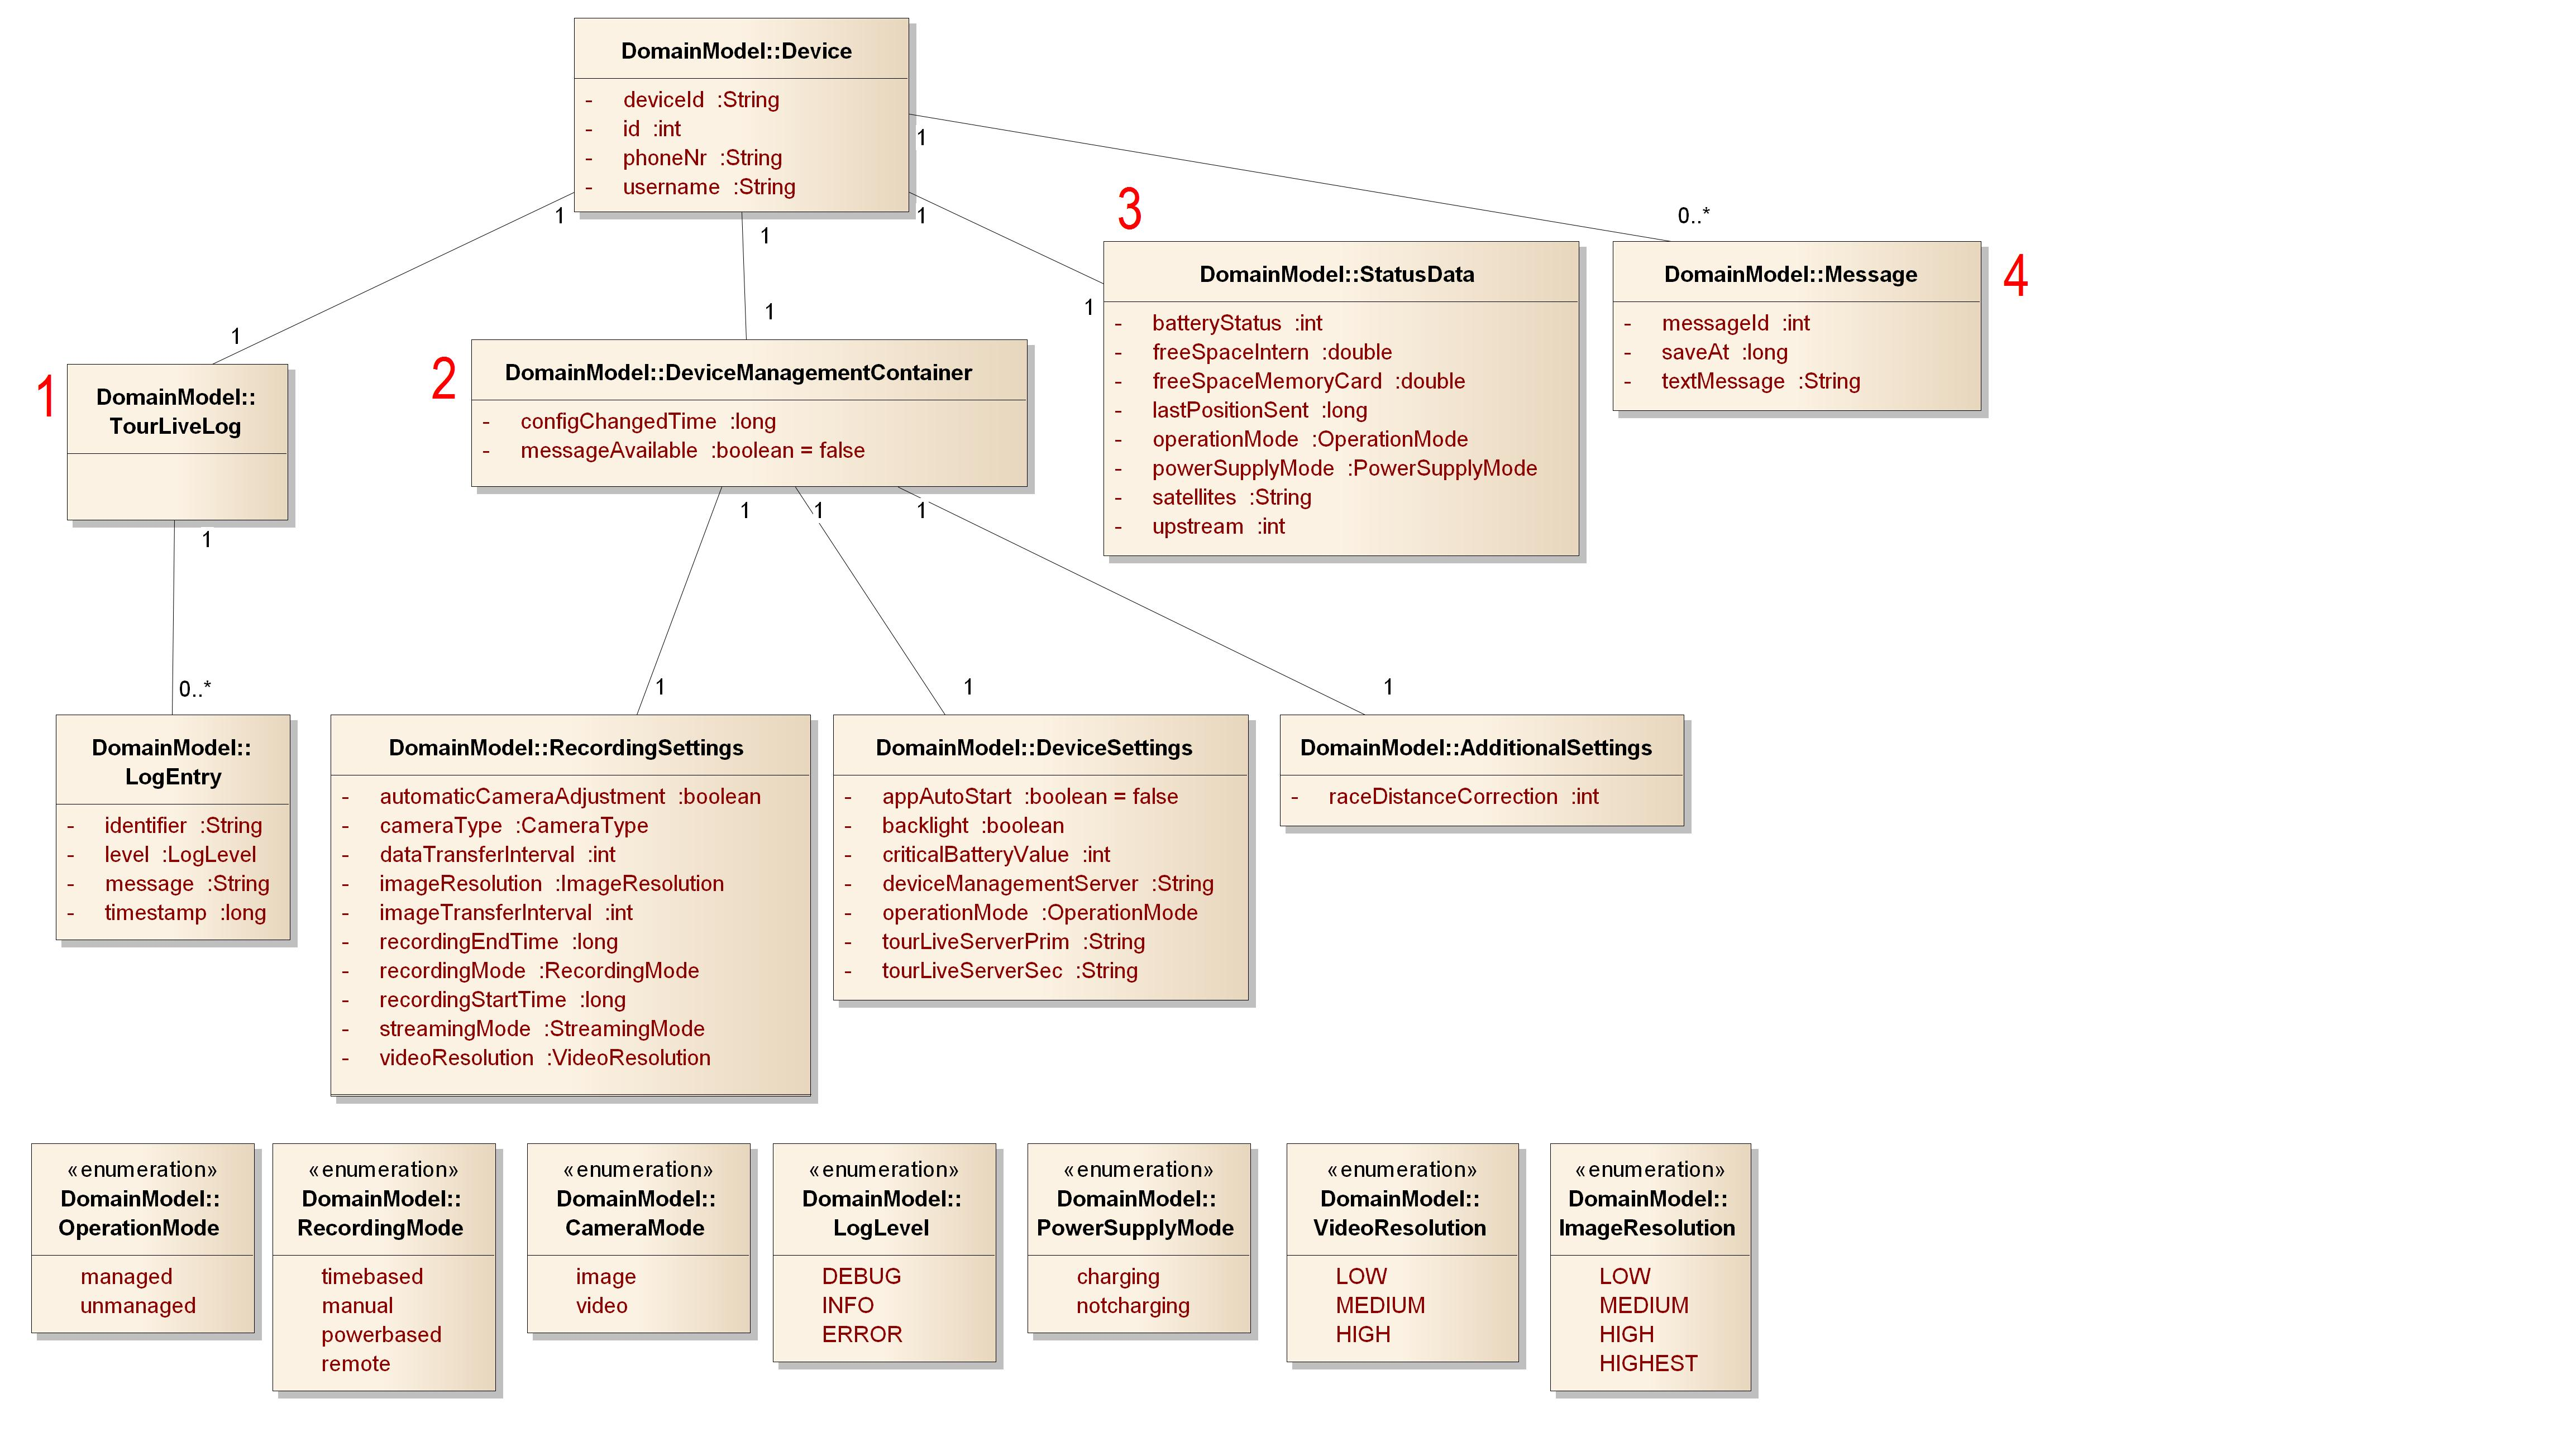
\includegraphics[width=120mm]{images/devmgmtsrv/domainmodel.jpg}
	\caption{Domain Model des Device Management Servers}
\end{figure}


\section{Software Design}
\subsection{Architektur und Übersicht}
Der Device Management Server hat zwei Hauptaufgaben. Zum einen wird die Bearbeitung der Daten ermöglicht und zum anderen wird dem Aufnahmesystemen eine API zur Verfügung gestellt.


\begin{figure}[H]
	\centering
	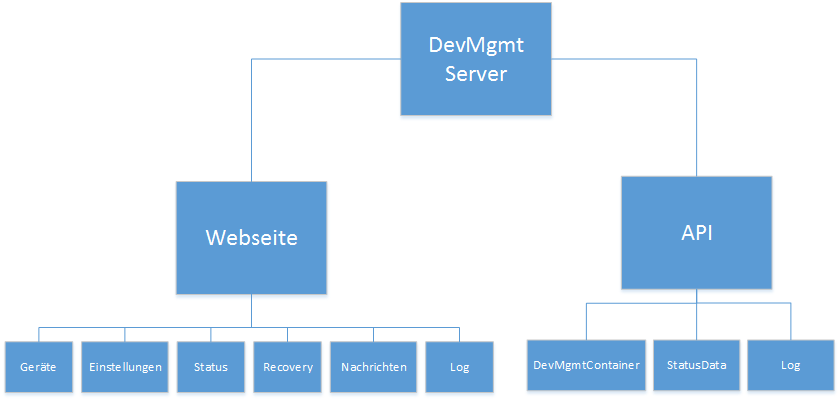
\includegraphics[width=120mm]{images/devmgmtsrv/uebersicht.png}
	\caption{Grobstruktur des Device Management Servers}
\end{figure}

Wie beim TourLive Server besteht dank der gewählten Struktur die Möglichkeit, die Webseite und die API auf verschiedene Server aufzuteilen. Da die Auslastung des Device Management Servers jedoch gering ist, wird darauf nicht weiter eingegangen.

\subsection{Schichtenmodell und Paketdiagramm}
Der Device Management Server ist in vier Schichten unterteilt. Die Schichten wurden an die Struktur des Spring Frameworks angepasst. Folgende Abbildung zeigt diese vier Schichten auf.

\begin{figure}[H]
	\centering
	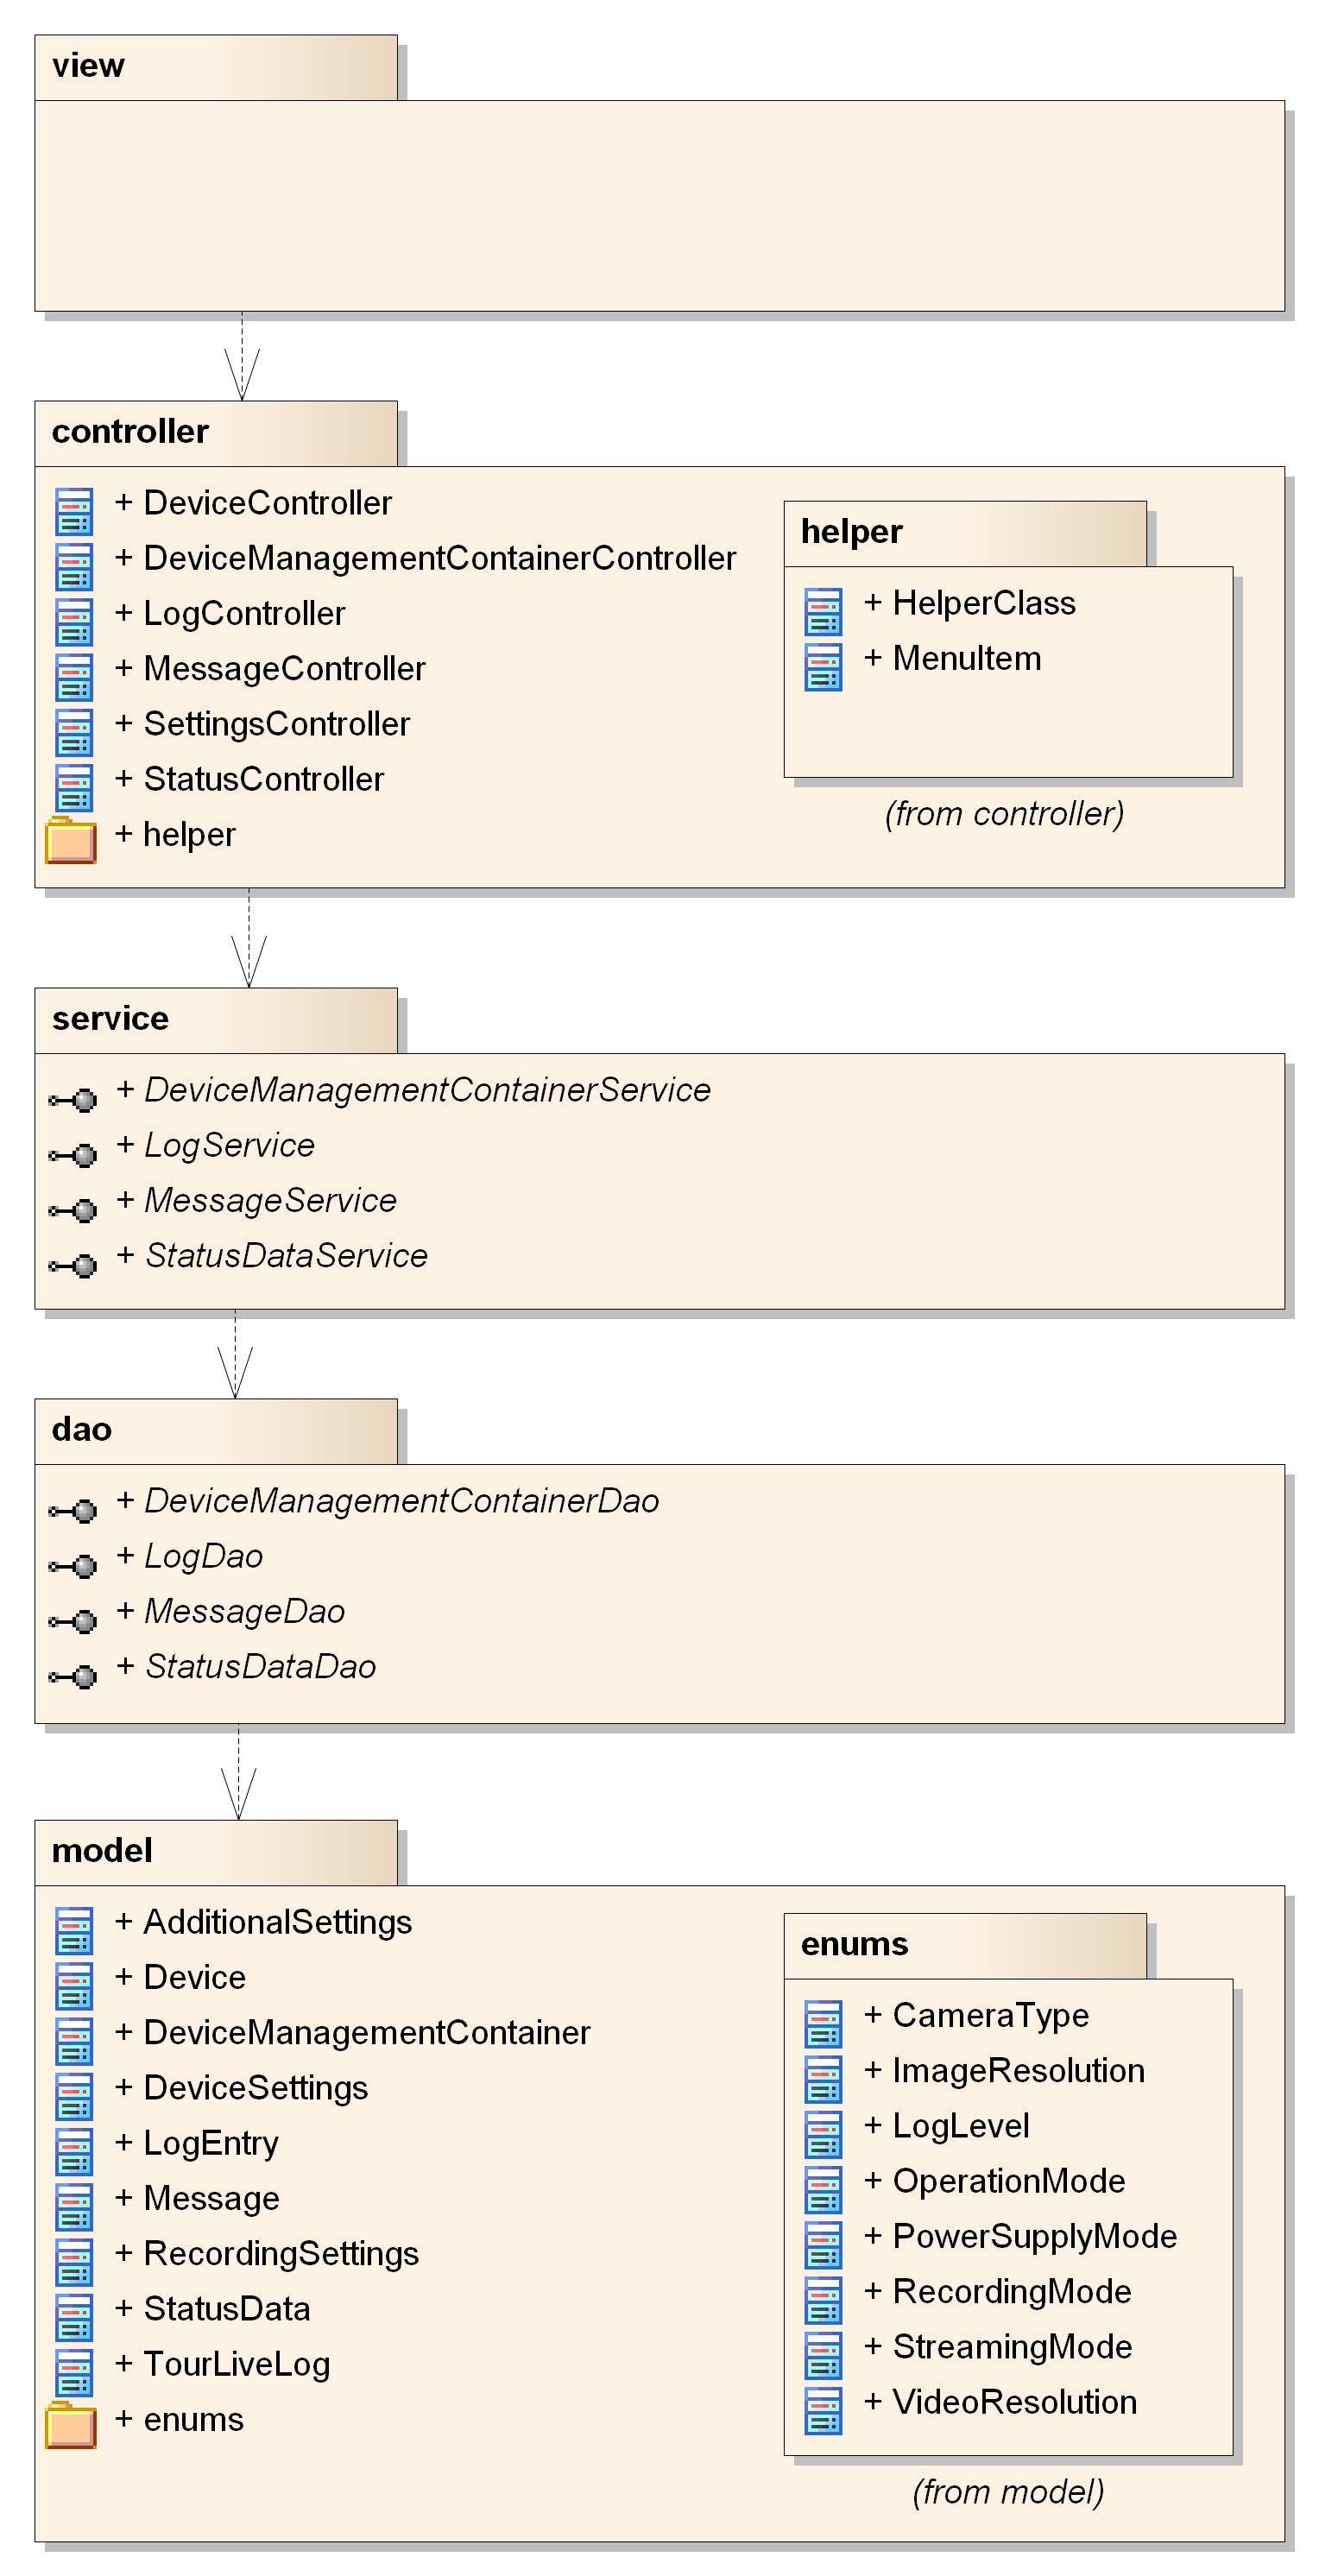
\includegraphics[width=80mm]{images/devmgmtsrv/schichten.jpg}
	\caption{Schichtendiagramm des Device Management Servers}
\end{figure}

\subsubsection{View}
Die View Schicht enthält alle *.jsp Dateien, die für die Darstellung der Webseite benötigt werden. 

\subsubsection{Controller}
Die Controller widerspiegeln die HTTP-Methoden (GET, POST,...) die für die Anzeige der Webseite und die RESTful JSON-Schnittstelle benötigt werden.

\subsubsection{Service}
Die Service Klassen sind für die Businesslogik auf den von den DAO's gelieferten Objekten verantwortlich.

\paragraph{DeviceManagementContainerService}
Der Device Management Container Service speichert und liefert die Container mit den Geräteeinstellungen sowie das Flag \textit{'messageAvailable'} falls auf dem Device Management Portal eine Nachricht für das Gerät vorhanden ist.

\subsubsection{DAO}
Die DAO Schicht enthält die Datenzugriffsobjekte. Diese dient zur Entkopplung der Geschäftslogik vom Datenzugriff. Die Interfaces bilden die Schnittstelle, die Implementierung kann so je nach Persistenztechnologie unterschiedlich sein, ohne dass die Geschäftslogik geändert werden muss.


\subsubsection{Model}
Die Domäne des Device Management Servers wird in der Model Schicht abgebildet. In den Objektinstanzen der Model Klassen sind die eigentlichen Daten gespeichert. Diese Objektinstanzen werden über den OR-Mapper in der SQL-Datenbank gespeichert.

\subsection{Device Management Container}
Der Device Management Container ist der wichtigste Teil des Device Management Servers. Er enthält alle Einstellungen für ein spezifisches Gerät. Es folgt ein Beispiel eines solchen Containers in JSON Notation.

\begin{figure}[H]
	\centering
	\lstinputlisting[language=json]{jsonfiles/settings.json}
	\caption{Einstellungen JSON}
\end{figure}



\section{Realisierung}
Folgendes Kapitel beschreibt die Umsetzung des Device Management Servers.

\subsection{API}
Die API wird mittels Spring Annotations definiert. 

\begin{lstlisting}[language=Java, caption=Spring Annotation]
@RequestMapping(value = "/api/getdevmgmtcontainer", method = RequestMethod.POST)
@ResponseBody
public DeviceManagementContainer getDeviceManagementContainer(@RequestBody final StatusData request)

\end{lstlisting}
\textbf{\textit{@RequestMapping}:} gibt an, welche URL auf diese Methode gemappt wird und welche Request Methode erlaubt ist.\\
\textbf{\textit{@ResponseBody}: } definiert, dass die Methode eine Antwort zurück gibt.\\
\textbf{\textit{@RequestBody}: } der Parameter der Methode wird als Body des Requests definiert.\\
Diese annotierten Methoden müssen in einer Klasse enthalten sein, welche als \textit{@Controller} annotiert ist.


\subsection{Webseite}
Die Webseiten wurden mit JSP umgesetzt. Als Erweiterung wurde Javascript sowie das JQuery Plugin verwendet. Um die grafische Oberfläche möglichst einfach zu gestalten, wurde das Twitter Bootstrap \footnote{Twitter Bootstrap, \url{http://twitter.github.io/bootstrap/}, besucht am 25. Mai 2013} CSS benutzt.

Die Webseite wird in drei Teile unterteilt, Header, Footer sowie der Hauptbereich. 

\begin{figure}[H]
	\centering
	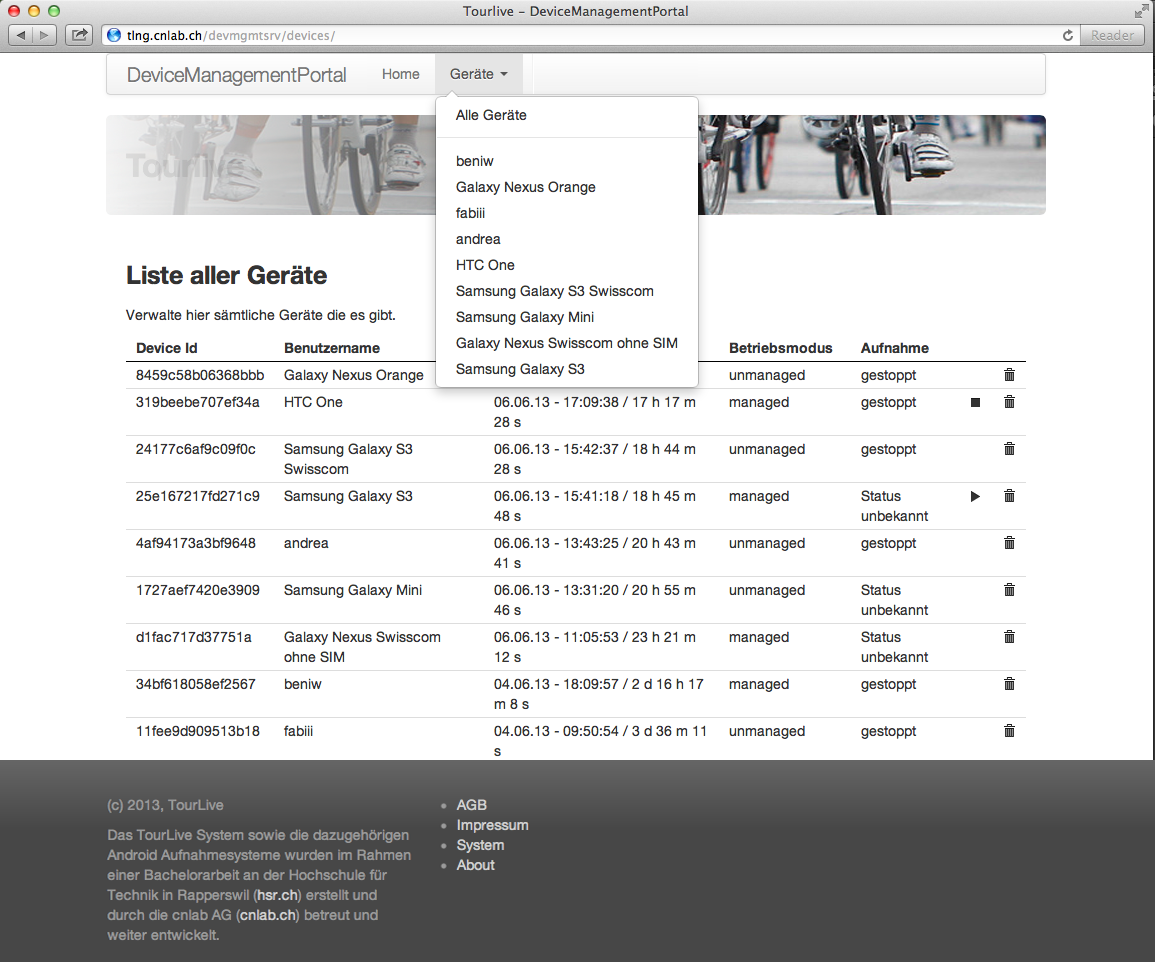
\includegraphics[width=120mm]{images/devmgmtsrv/all.png}
	\caption{Übersicht der DevMgmt Webseite}
\end{figure}

\subsubsection{Header}
Der Header bietet die Möglichkeit, über eine Schnellnavigation auf ein Gerät zuzugreifen. 
\begin{figure}[H]
	\centering
	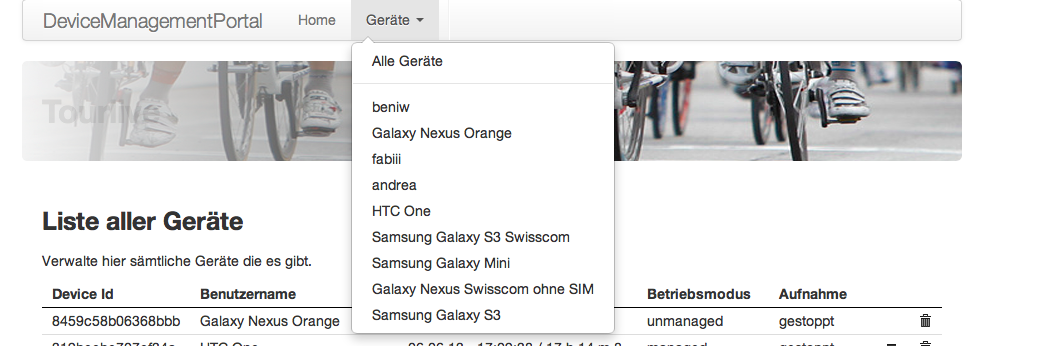
\includegraphics[width=120mm]{images/devmgmtsrv/header.png}
	\caption{DevMgmt Webseite Header}
\end{figure}



\subsubsection{Footer}
Der Footer enthält detaillierte Informationen zum Projekt TourLive. 
 
\begin{figure}[H]
	\centering
	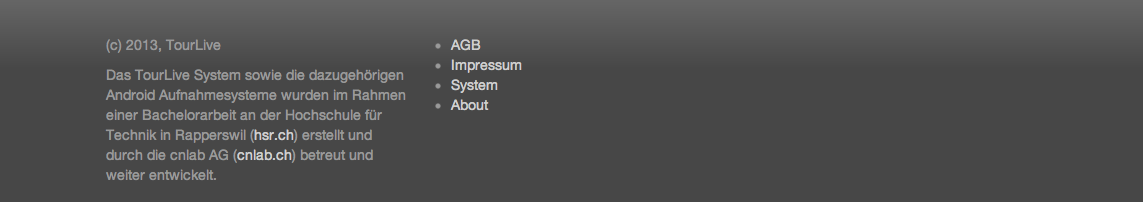
\includegraphics[width=120mm]{images/devmgmtsrv/footer.png}
	\caption{DevMgmt Webseite Footer}
\end{figure}


\subsubsection{Hauptbereich}
Der Hauptbereich unterteilt sich wieder in zwei Teile. So hat man Links eine neue Navigation, mit welcher man sich zwischen den verschiedenen Seiten hin und her bewegen kann. 
 
\begin{figure}[H]
	\centering
	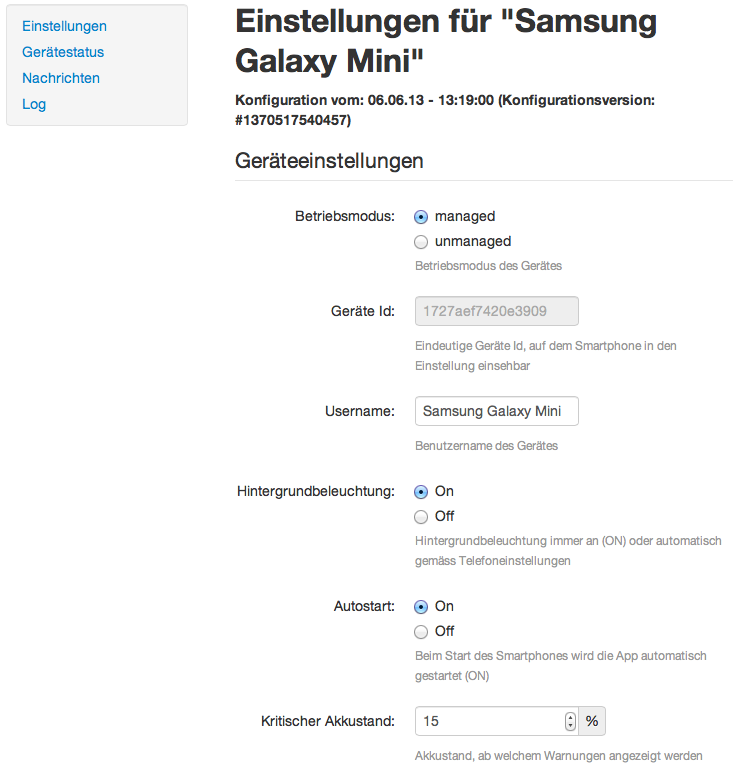
\includegraphics[width=120mm]{images/devmgmtsrv/settings.png}
	\caption{DevMgmt Webseite Hauptbereich}
\end{figure}

\subsection{Datenbank}
Die Speicherung der Daten in der Datenbank erfolgt mittels Hibernate Annotations.

\begin{lstlisting}[language=Java, caption=Hibernate Annotation]
@Entity
@Table(name = "Device")
public class Device {
	@Id
	@Column(name = "deviceId")
	private String deviceId;
	@Column
	private String username;
	@Column
	private String phoneNr;
}
\end{lstlisting}

\textbf{\textit{@Entity}:} mit dieser Annotation wird angegeben, dass diese Klasse eine gemappte Hibernate Klasse ist.\\
\textbf{\textit{@Table}:} optional, bei der Angabe dieses Attributs, kann der Name der Tabelle definiert werden.\\
\textbf{\textit{@Id}:} definiert das folgende Attribut als Primärschlüssel.\\
\textbf{\textit{@Column}:} das folgende Attribut definiert die Spalte.
